\documentclass[12pt]{beamer}
\usepackage[utf8]{inputenc}
\usepackage[T1]{fontenc}
\usepackage{lmodern}
\usepackage{amsmath}
\usepackage{amsfonts}
\usepackage{amssymb}
\usepackage{hyperref}
\usepackage{graphicx}
\usepackage{listings}

\definecolor{links}{HTML}{2A1B81}
\hypersetup{colorlinks,linkcolor=,urlcolor=links}
\usetheme{Boadilla}
\setbeamertemplate{footline}[frame number]

\begin{document}
	\author{Group A}
	\title{SEEMATH}
	\subtitle{math visualization website}
	%\logo{}
	\institute{Department of Mathematics \\ Kathmandu University}
	\date{\today}
	%\subject{}
	\setbeamercovered{transparent}
	\setbeamertemplate{navigation symbols}{}
	
	\begin{frame}[plain]
		\maketitle
	\end{frame}
	
	%mukeshssss
	\begin{frame}{}	
	\begin{minipage}{0.25\linewidth}
		\noindent
		\textbf{ Introduction}\\
		\vspace{1cm}
		Static Website\\
		with\\
		Interactive \\
		Demos 
		\vspace{8cm}	\end{minipage}
	\begin{minipage}{0.7\linewidth}
	\begin{figure}
	\centering
	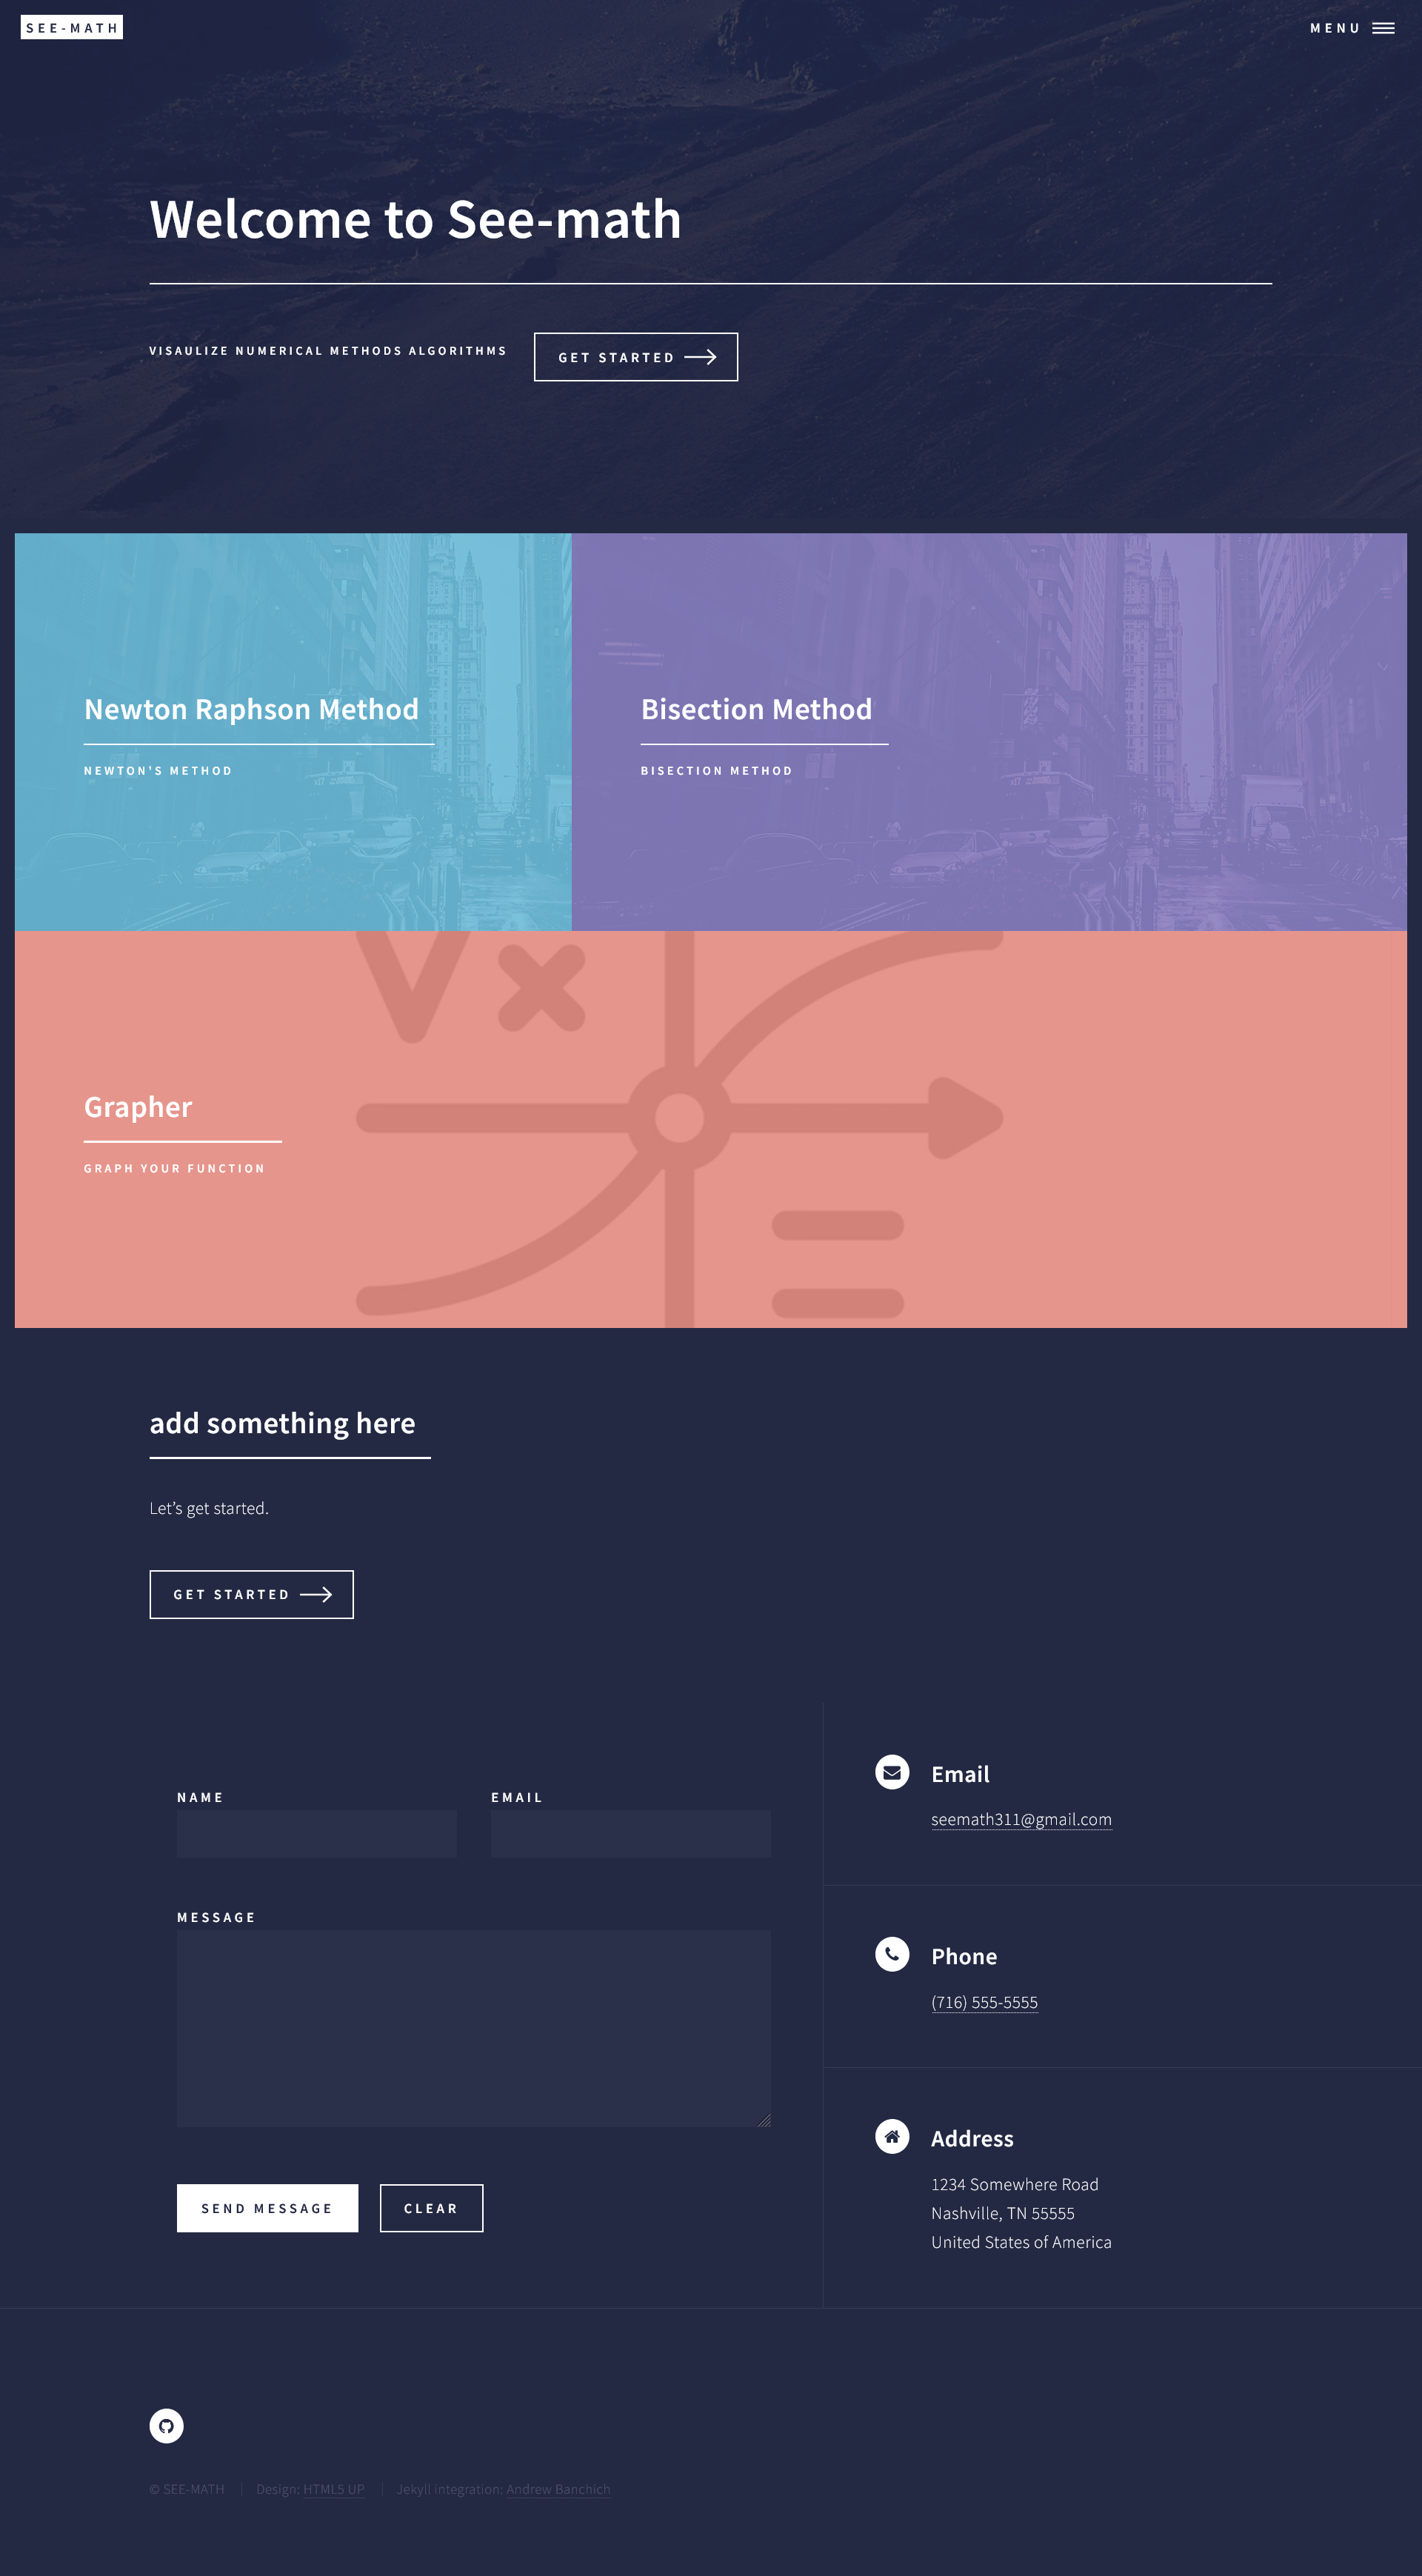
\includegraphics[width=0.95\linewidth]{seemath1}
	\label{fig:seemath1}
\end{figure}
\end{minipage}
\end{frame}
	.
	%bishesh
	
\begin{frame}{Timeline}
Below figure shows the plan we had and how the workflow was executed.
\begin{figure}[ht]
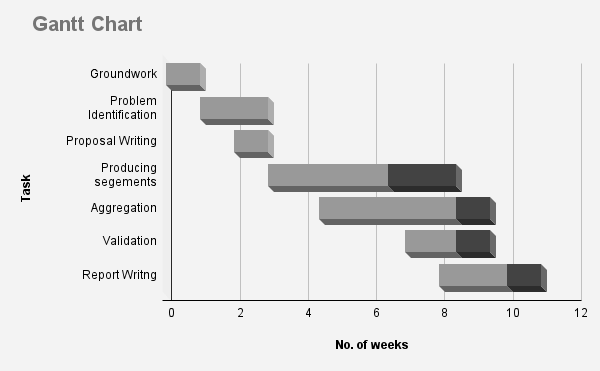
\includegraphics[width = 7cm]{GanttChart.png}
\caption{\textbf{Gray:} Estimated duration; \textbf{Black:} Actual Duration}
\end{figure}
\end{frame}


	%objectives
	\begin{frame}{Objectives}
\begin{block}{Primary Objectives}
\begin{itemize}
    \item To be able to have step by step visualization for numerical method algorithms.
    \item To have a user interactive platform for teaching and learning aid.
\end{itemize}
\end{block}
\begin{block}{Secondary Objectives:}
\begin{itemize}
    \item Learn Web Development Frame work including back-end and front-end.
    \item Learning to build mathematical animations and interactive plots.
\end{itemize}
\end{block}
\end{frame}


	
	%parena
	\begin{frame}{Demonstration}
		\url{https://see-math.github.io/}
	\end{frame}

	
\begin{frame}{Features}
Till date, the following features have been integrated on our website:
\begin{itemize}
    \item Grapher : Plots the given function.
    \item Bisection Method
    \item Newton-Raphson Method
    \item A message form for interaction.
\end{itemize}
\end{frame}

		\begin{frame}{Limitations}
		\begin{itemize}
			
			\item {Only  Bisection method and newton raphson method upto now.}
			
			\item {Few edge cases need to be resolved.}
			
			
			
		\end{itemize}
		
	\end{frame}
	%prajanya
	\begin{frame}{Future Plans}
\begin{itemize}
	
	\item {Adding various methods and enhancing the current model.}
	
	\item {To explore the latest web technologies to build a highly functional future proof website with longevity built-in.}
	
	\item {Making the website as user friendly and interactive as possible.}
	
\end{itemize}
	\end{frame}

	%priyanka
	\begin{frame}{References and Acknowledgment}
     \begin{figure}
     	\centering
     	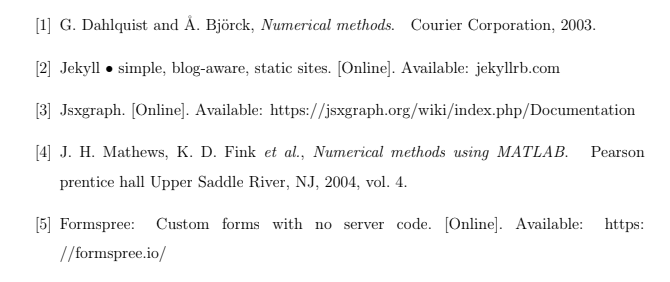
\includegraphics[width=0.95\linewidth]{ref.png}
    
     \end{figure}
		
\end{frame}
		\begin{frame}{ Acknowledgment}


\begin{itemize}
	\item \textbf{Prof. Dr. Samir Shrestha}\\ 
	
	Department of Mathematics


	\item \textbf{Mr. Amrit Dahal}\\Department of Computer Science and Engineering
\end{itemize}

	\end{frame}
\end{document}